%\documentclass[10pt,notheorems]{beamer}
%\documentclass{beamer} % version for playing slides
\documentclass[handout,10pt]{beamer} % version for print
%\usepackage{xeCJK}
\usepackage{ctex}
%\usepackage{eucal} % for \mathcal
%\usepackage[linewidth=1pt]{mdframed} % for  mdframe environment


 % 1. packages

 % ----------- fonts and symbles ---------
\usepackage{amsmath,amssymb,amsfonts,amsthm}
%\usepackage{CJK}
\usepackage{dsfont}
\usepackage{mathrsfs}
\usepackage{eucal} % for \mathcal

%\renewcommand{\rmdefault}{ptm}


%\usepackage{fontspec}
%\newfontfamily\monaco{Monaco}

%\usepackage{mathbbold} %,bbold

 \usepackage{textcomp} % for \textnormal{\textperthousand}
% -----------------





%\usepackage{slashbox}
%\usepackage[margin=2.2cm]{geometry} % |geometry| package clash with |booktabs| package
%\usepackage{cases}
% -------- tables -------
\usepackage{booktabs} % for \toprule, \bottomrule
\usepackage{tabularx}
\usepackage{multirow}
% --------- figures ---------
\usepackage{graphicx}
% ---------- algorithms -------
\usepackage{algorithm}
\usepackage{algorithmic}
%\usepackage{footnote}
    % |footnote| package occurs error:
    % Runaway argument?
    % \def \insertfootnotetext {\@@ }\def \insertfootnotemark {\@makefnmark \ETC.

\usepackage{listings}

\usepackage[linewidth=1pt]{mdframed} % for  mdframe environment




 \usepackage{color}
 \usepackage{xcolor}     %¸ßÁÁʹÓõÄÑÕÉ«

\usepackage{setspace}
%%\usepackage{type1cm}
\usepackage{adjustbox} % for \adjustbox

\usepackage{accsupp}
\newcommand{\emptyaccsupp}[1]{\BeginAccSupp{ActualText={}}#1\EndAccSupp{}}




%%   figures and tables
\graphicspath{{figure/}}


% 2. new commands

% 2.0 common commands
%\newcommand{\bc}{\begin{center}}
%\newcommand{\ec}{\end{center}}
%\newcommand{\ba}{\begin{array}}
%\newcommand{\ea}{\end{array}}
%\newcommand{\be}{\begin{equation}}
%\newcommand{\ee}{\end{equation}}

% 2.1 colors
\definecolor{dgrey}{rgb}{0.30,0.30,0.30}
\definecolor{lred}{rgb}{0.50,0.00,0.50}
\definecolor{lblue}{rgb}{0.8,0.8,1}
\definecolor{dred}{rgb}{0.6,0,0}
\definecolor{dblue}{rgb}{0,0,0.5}
\definecolor{dgrey}{rgb}{0.35,0.35,0.35}
\definecolor{rred}{rgb}{0.9,0,0}
\definecolor{mylblue}{rgb}{0.3,0.2, 0.8}

\definecolor{commentcolor}{RGB}{85,139,78}
\definecolor{stringcolor}{RGB}{206,145,108}
\definecolor{keywordcolor}{RGB}{34,34,250}
\definecolor{backcolor}{RGB}{220,220,220}

\newcommand{\blue}[1]{{\color{blue}#1}}
\newcommand{\dblue}[1]{{\color{dblue}#1} }
\newcommand{\red}[1]{{\color{red}#1}}
\newcommand{\dred}[1]{{\color{dred}#1}}
\newcommand{\cyan}[1]{{\color{cyan}#1}}
\newcommand{\bfblue}[1]{\textbf{\color{dblue}#1} }
\newcommand{\bfred}[1]{\textbf{\color{dred}#1} }
\newcommand{\green}[1]{{\color{green}#1}}
%\newcommand{\alert}[1]{{\color{red}#1}}
\newcommand{\black}[1]{{\color{black}#1}}
\newcommand{\light}[1]{{\color{blue}\textbf{#1}}}
\newcommand{\hot}[1]{{\color{dred}#1}}
 \newcommand{\highlight}[1]{ \textbf{\color{mylblue}#1}}
 \newcommand{\important}[1]{{\color{red}#1}} % for highlighting  some words

 \newcommand{\mystar}{\dred{$^{\clubsuit}$ }}
  \newcommand{\doublestar}{\dred{$^{\clubsuit\clubsuit}$ }}

\newcommand{\mynote}[1]{{\footnotesize \color{mylblue}#1}}

 \newcommand{\hint}[1]{{\small \color{mylblue}#1}}
\newcommand{\smallhint}[1]{{\small \color{dgrey}#1}}
\newcommand{\footnotehint}[1]{{\footnotesize \color{dgrey}#1}}
\newcommand{\tinyhint}[1]{{\tiny \color{dgrey}#1}}
\newcommand{\mytitle}[1]{\medskip{\large \textbf{\color{mylblue}#1}}}
\newcommand{\normaltitle}[1]{\medskip{ \textbf{\color{mylblue}#1}}}

%\newcommand{\head}[1]{\textbf{\large\color{blue}#1}}
%\newcommand{\heading}[1]{\textbf{\large\color{blue}#1}}

\newcommand{\myfbox}[2]{ \bigskip \begin{center} \fbox{\parbox{#1}{ #2  }} \end{center}\bigskip }

\newcommand{\myvar}[1]{}
%\newcommand{\mynote}[1]{#1}

% 2.2 mathematical symbols

\newcommand{\drightarrow}{\stackrel{d.}{\rightarrow}}
\newcommand{\prightarrow}{\stackrel{p.}{\rightarrow}}
\newcommand{\bernoulli}{\textnormal{Ber}}
\newcommand{\cov}{\mathsf{Cov}}
\newcommand{\corr}{\mathbf{Corr}}
\newcommand{\regret}{\textnormal{Regret}}
\newcommand{\conv}{\textnormal{conv}}
\newcommand{\dotdiv}{\stackrel{\centerdot}{-}}
\newcommand{\dom}{\textnormal{dom}}
\newcommand{\convergenceinprob}{\stackrel{P}{\rightarrow}}
\newcommand{\convergenceindist}{\rightsquigarrow}
\newcommand{\probability}{\mathbb{P}}
\newcommand{\expectation}{\mathbb{E}}
\newcommand{\epi}{\textnormal{epi}}
\newcommand{\variance}{\mathbb{V}}
\newcommand{\var}[1]{\mathbb{V}(#1)}
\newcommand{\covariance}{\mathsf{Cov}}
\newcommand{\empiricalrisk}[1]{\hat{R}(#1)}
\newcommand{\expectedrisk}[1]{R(#1)}
\newcommand{\mgf}[1]{\psi_{#1}(\lambda)}
\newcommand{\mgfexpansion}[1]{\expectation[e^{\lambda#1}]}
\newcommand{\mgfmultivariate}[1]{\expectation[e^{\lambda^\transpose#1}]}
\newcommand{\transpose}{{\mathsf{T}}}
\newcommand{\real}{\mathbb{R}}
\newcommand{\gaussian}[2]{\mathcal{N}(#1,#2)}
\newcommand{\subGaussian}[1]{\mathsf{subG}(#1)}
\newcommand{\indicator}[1]{\mathbb{I}[#1]}
\newcommand{\x}[1]{x^{(#1)}}
\newcommand{\y}[1]{y^{(#1)}}
\newcommand{\z}[1]{z^{(#1)}}
\newcommand{\feature}{x}
\newcommand{\response}{y}
\newcommand{\supofempiricalprocess}{\|\mathbb{P}_n-\mathbb{P}\|_{\decisionspace}}
\newcommand{\decisionspace}{\mathscr{F}}
\newcommand{\decisionfunction}{f}
\newcommand{\featurespace}{\mathcal{X}}
\newcommand{\classifierestimate}{\widehat{h}}
\newcommand{\classifiertrue}{h^\star}
\newcommand{\classifier}{h}
\newcommand{\hypothesisclass}{\mathcal{H}}
\newcommand{\dataset}{\mathcal{D}}
\newcommand{\defineas}{\stackrel{\textnormal{def}}{=}}
\newcommand{\rademachercomplexity}[1]{\mathsf{Rad}_n\left(#1\right)}
\newcommand{\loss}{\ell}
\newcommand{\composite}{\circ}
\newcommand{\convexhull}{\mathsf{conv}}
\newcommand{\norm}[2][2]{\|#2\|_{#1}}
\newcommand{\shatteringcoefficient}[2]{\mathcal{S}(#1,#2)}
\newcommand{\vcdimension}[1]{\mathsf{VC}\left(#1\right)}
\newcommand{\rank}{\mathsf{rank}}
\newcommand{\innerproduct}[2]{\left\langle #1, #2\right\rangle}
\newcommand{\modelparameter}{\theta}
\newcommand{\ball}[3][]{\mathcal{B}_{{#1}}\left(#2,#3\right)}
\newcommand{\metric}{d}
\newcommand{\coveringnumber}[4][]{N_{{#1}}\left(#2,#3,#4\right)}
\newcommand{\trace}{\textnormal{tr}}
\newcommand{\std}{\textnormal{std}}
\newcommand{\sgn}{\textnormal{sign}}
%\renewcommand{\span}{\textnormal{span}}

 % do not overwrite the existing command \span
 % as it leads to an error of
 %  "Missing # Inserted in Alignment Preamble" for ``align'' environment

\newcommand{\myspan}{\textnormal{span}}

%%%
\newcommand{\rightarrowd}{\stackrel{d}{\rightarrow}}
\newcommand{\rightarrowp}{\stackrel{p}{\rightarrow}}
\newcommand{\defeq}{ \stackrel{\textnormal{def}}{=}}
\newcommand{\proj}{ \textnormal{Proj}}
\newcommand{\dist}{\textnormal{dist}}

\newcommand{\argmax}{\textnormal{argmax}}
\newcommand{\argmin}{\textnormal{argmin}}
\newcommand{\subg}{\textnormal{subG}}


 \newcommand{\bba}{\mathbb{A}}
\newcommand{\bbb}{\mathbb{B}}
\newcommand{\bbc}{\mathbb{C}}
\newcommand{\bbd}{\mathbb{D}}
\newcommand{\bbe}{\mathbb{E}}
\newcommand{\bbf}{\mathbb{F}}
\newcommand{\bbg}{\mathbb{G}}
\newcommand{\bbh}{\mathbb{H}}
\newcommand{\bbi}{\mathbb{I}}
\newcommand{\bbj}{\mathbb{J}}
\newcommand{\bbk}{\mathbb{K}}
\newcommand{\bbl}{\mathbb{L}}
\newcommand{\bbm}{\mathbb{M}}
\newcommand{\bbn}{\mathbb{N}}
\newcommand{\bbo}{\mathbb{O}}
\newcommand{\bbp}{\mathbb{P}}
\newcommand{\bbq}{\mathbb{Q}}
\newcommand{\bbr}{\mathbb{R}}
\newcommand{\bbs}{\mathbb{S}}
\newcommand{\bbt}{\mathbb{T}}
\newcommand{\bbu}{\mathbb{U}}
\newcommand{\bbv}{\mathbb{V}}
\newcommand{\bbw}{\mathbb{W}}
\newcommand{\bbx}{\mathbb{X}}
\newcommand{\bby}{\mathbb{Y}}
\newcommand{\bbz}{\mathbb{Z}}

\newcommand{\bfa}{\mathbf{a}}
\newcommand{\bfb}{\mathbf{b}}
\newcommand{\bfc}{\mathbf{c}}
\newcommand{\bfd}{\mathbf{d}}
\newcommand{\bfe}{\mathbf{e}}
\newcommand{\bff}{\mathbf{f}}
\newcommand{\bfg}{\mathbf{g}}
\newcommand{\bfh}{\mathbf{h}}
\newcommand{\bfi}{\mathbf{i}}
\newcommand{\bfj}{\mathbf{j}}
\newcommand{\bfk}{\mathbf{k}}
\newcommand{\bfl}{\mathbf{l}}
\newcommand{\bfm}{\mathbf{m}}
\newcommand{\bfn}{\mathbf{n}}
\newcommand{\bfo}{\mathbf{o}}
\newcommand{\bfp}{\mathbf{p}}
\newcommand{\bfq}{\mathbf{q}}
\newcommand{\bfr}{\mathbf{r}}
\newcommand{\bfs}{\mathbf{s}}
\newcommand{\bft}{\mathbf{t}}
\newcommand{\bfu}{\mathbf{u}}
\newcommand{\bfv}{\mathbf{v}}
\newcommand{\bfw}{\mathbf{w}}
\newcommand{\bfx}{\mathbf{x}}
\newcommand{\bfy}{\mathbf{y}}
\newcommand{\bfz}{\mathbf{z}}

\newcommand{\bfA}{\mathbf{A}}
\newcommand{\bfB}{\mathbf{B}}
\newcommand{\bfC}{\mathbf{C}}
\newcommand{\bfD}{\mathbf{D}}
\newcommand{\bfE}{\mathbf{E}}
\newcommand{\bfF}{\mathbf{F}}
\newcommand{\bfG}{\mathbf{G}}
\newcommand{\bfH}{\mathbf{H}}
\newcommand{\bfI}{\mathbf{I}}
\newcommand{\bfJ}{\mathbf{J}}
\newcommand{\bfK}{\mathbf{K}}
\newcommand{\bfL}{\mathbf{L}}
\newcommand{\bfM}{\mathbf{M}}
\newcommand{\bfN}{\mathbf{N}}
\newcommand{\bfO}{\mathbf{O}}
\newcommand{\bfP}{\mathbf{P}}
\newcommand{\bfQ}{\mathbf{Q}}
\newcommand{\bfR}{\mathbf{R}}
\newcommand{\bfS}{\mathbf{S}}
\newcommand{\bfT}{\mathbf{T}}
\newcommand{\bfU}{\mathbf{U}}
\newcommand{\bfV}{\mathbf{V}}
\newcommand{\bfW}{\mathbf{W}}
\newcommand{\bfX}{\mathbf{X}}
\newcommand{\bfY}{\mathbf{Y}}
\newcommand{\bfZ}{\mathbf{Z}}


\newcommand{\bfSigma}{\mathbf{\Sigma}}
\newcommand{\bfrho}{\mathbf{\rho}}

\newcommand{\cala}{\mathcal{A}}
\newcommand{\calb}{\mathcal{B}}
\newcommand{\calc}{\mathcal{C}}
\newcommand{\cald}{\mathcal{D}}
\newcommand{\cale}{\mathcal{E}}
\newcommand{\calf}{\mathcal{F}}
\newcommand{\calg}{\mathcal{G}}
\newcommand{\calh}{\mathcal{H}}
\newcommand{\cali}{\mathcal{I}}
\newcommand{\calj}{\mathcal{J}}
\newcommand{\calk}{\mathcal{K}}
\newcommand{\call}{\mathcal{L}}
\newcommand{\calm}{\mathcal{M}}
\newcommand{\caln}{\mathcal{N}}
\newcommand{\calo}{\mathcal{O}}
\newcommand{\calp}{\mathcal{P}}
\newcommand{\calq}{\mathcal{Q}}
\newcommand{\calr}{\mathcal{R}}
\newcommand{\cals}{\mathcal{S}}
\newcommand{\calt}{\mathcal{T}}
\newcommand{\calu}{\mathcal{U}}
\newcommand{\calv}{\mathcal{V}}
\newcommand{\calw}{\mathcal{W}}
\newcommand{\calx}{\mathcal{X}}
\newcommand{\caly}{\mathcal{Y}}
\newcommand{\calz}{\mathcal{Z}}


% 3. theorem and environments

%\newtheorem{theorem}{Theorem}%[section]
\newtheorem{proposition}{Proposition}%[section]
%\newtheorem{property}{Property}%[section]
%\newtheorem{lemma}{Lemma}%[section]
%\newtheorem{corollary}{Corollary}%[section]
%\newtheorem{definition}{Definition}%[section]
%\newtheorem{example}{Example}%[section]
%\newtheorem{remark}{Remark}%[section]
%\newtheorem{note}{Note}%[section]
%\newtheorem{problem}{Problem}%[section]
\newtheorem{exercise}{Exercise}
%\newtheorem{assumption}{Assumption}
\newtheorem*{lemma_star}{Lemma}
\newtheorem*{theorem_star}{Theorem}

%\newenvironment{summary}[1][Summary]{\par\medskip   \color{dred}\textbf{\large#1. } }{ \medskip}
%\newenvironment{remark}[1][Remark]{\par\medskip  \begin{small} \color{dblue}\textbf{#1. } }{ \end{small}\medskip}
%\renewenvironment{proof}[1][Proof]{\noindent\textbf{#1.} }{\mbox{} \hfill{\small\textrm{$\Box$}}\vspace{1ex}}
% \newenvironment{answer}[1][Answer]{\par\medskip \color{dblue}\textbf{\large#1. }}{ \medskip}

\newenvironment{summary}[1][总结]{\par\medskip   \color{dred}\textbf{\large#1 } }{ \medskip}
\newenvironment{remark}[1][注意]{\par\medskip   \color{dblue}\textbf{\large#1 } }{ \medskip}
\newenvironment{footnoteremark}{ \color{dblue}\begin{footnotesize} }{\end{footnotesize}}
\renewenvironment{proof}[1][证明]{\noindent\textbf{#1.} }{\mbox{} \hfill{\small\textrm{$\Box$}}\vspace{1ex}}
 \newenvironment{question}[1][Q.]{\par\medskip {\color{lred}\large#1}}{ \medskip}
 \newenvironment{answer}[1][Answer]{\par\medskip \color{dblue}\textbf{\large#1 }}{ \medskip}

% 4. beamer setting




%\newtheorem{definition}{\textbf{¶¨Òå}}[section]
%\newtheorem{proposition}[definition] { \textbf{ÃüÌâ}}
%\newtheorem{lemma}[definition] { \textbf{ÒýÀí}}
%\newtheorem{theorem}[definition]{ \textbf{¶¨Àí}}
%\newtheorem{corollary}[definition] { \textbf{ÍÆÂÛ}}
%\newtheorem{remark}[definition] { \textbf{×¢}}
%\newtheorem{example}[definition] { \textbf{Àý}}

%\newcommand{\shadow}[1]{\begin{center}
%\bf{\textcolor{dblue}{\shadowbox{\parbox{3.8in}
% {\textcolor{red}
% {\vspace{1mm}#1}}}}}
%\end{center}}
%
%\newcommand{\head}[1]{\begin{center}
%\bf{\textcolor{dblue}{\shadowbox{\parbox{3.8in}
% {\textcolor{dred}
% {\vspace{1mm}#1}}}}}
%\end{center}}
%
%
%\newcommand{\heading}[1]{%
%  \begin{center}
%    \large\bf
%    \shadowbox{#1}%
%  \end{center}
%\vspace{1ex minus 1ex}}

% set  space above and below math equations in display style

\expandafter\def\expandafter\normalsize\expandafter{%
    \normalsize
    \setlength\abovedisplayskip{1.5ex}
    \setlength\belowdisplayskip{1.2ex}
    \setlength\abovedisplayshortskip{0.5ex}
    \setlength\belowdisplayshortskip{0.5ex}
}

% Ìí¼ÓÒ³Âë´úÂ룬¹È¸èÕÒµ½µÄ¡£
\addtobeamertemplate{navigation symbols}{}{%
    %\usebeamerfont{footline}%
    %\usebeamercolor[fg]{footline}%
    \setbeamercolor{footline}{fg=blue}
    \setbeamerfont{footline}{series=\bfseries}
    \hspace{1em}%
    \normalsize{\insertframenumber/\inserttotalframenumber}
}

% section numbering
\setbeamertemplate{section in toc}[sections numbered]
\setbeamertemplate{subsection in toc}[subsections numbered]



\lstset{                        %¸ßÁÁ´úÂëÉèÖÃ
%basicstyle=\small, % print whole listing small
%basicstyle=\footnotesize\sffamily, % print whole listing small
basicstyle=\footnotesize\rmfamily, % print whole listing small
%basicstyle=\rmfamily, % print whole listing small
    language=python,                    %PythonÓï·¨¸ßÁÁ
    %linewidth=0.9\linewidth,            %Áбílist¿í¶È
    %basicstyle=\ttfamily,              %ttÎÞ·¨ÏÔʾ¿Õ¸ñ
    commentstyle=\color{commentcolor},  %×¢ÊÍÑÕÉ«
    keywordstyle=\color{keywordcolor},  %¹Ø¼ü´ÊÑÕÉ«
    stringstyle=\color{stringcolor},    %×Ö·û´®ÑÕÉ«
    %showspaces=true,                   %ÏÔʾ¿Õ¸ñ
    numbers=left,                       %ÐÐÊýÏÔʾÔÚ×ó²à
    %numberstyle=\tiny\emptyaccsupp,     %ÐÐÊýÊý×Ö¸ñʽ
    numberstyle=\tiny,                  %ÐÐÊýÊý×Ö¸ñʽ
    numbersep=5pt,                      %Êý×Ö¼ä¸ô
    frame=single,                       %¼Ó¿ò
    framerule=0pt,                      %²»»®Ïß
    %escapeinside=@@,                    %ÌÓÒݱêÖ¾
    escapeinside=``,                    %ÌÓÒݱêÖ¾
    emptylines=1,                       %
    xleftmargin=3em,                    %list×ó±ß¾à
    backgroundcolor=\color{backcolor},  %ÁÐ±í±³¾°É«
    tabsize=4,                          %ÖƱí·û³¤¶ÈΪ4¸ö×Ö·û
    %gobble=4                            %ºöÂÔÿÐдúÂëÇ°4¸ö×Ö·û
    breaklines=true,
    extendedchars=false
    }

\lstdefinestyle{numbers}{numbers=left, stepnumber=1, numberstyle=\tiny, numbersep=10pt}
 \lstdefinestyle{nonumbers}{numbers=none}

\newcommand{\alertcode}[1]{{\color{red}#1}} % used for alerting codes

%\lstset{numbers=left, numberstyle=\tiny,
%keywordstyle=\color{blue!70},
%commentstyle=\color{red!50!green!50!blue!50},
%frame=shadowbox,
%rulesepcolor=\color{red!20!green!20!blue!20},
%escapeinside=``,
%framesep = 2ex,
%rulesep = 1ex
%%framexrightmargin= 1em %
%}


% Vary the color applet  (try out your own if you like)
\colorlet{structure}{red!65!black}

%\beamertemplateshadingbackground{yellow!50}{white}


%\setbeamerfont{normal text}{family=\rmfamily}
%\setbeamerfont{frametitle}{family=\rmfamily}

% Changing the fonts: this will make the slides more readable and the math look like regular tex math
\usefonttheme{serif}



% set spaces

\setstretch{1.2}  % ÉèÖÃÐоà

\addtobeamertemplate{block begin}{\setlength\abovedisplayskip{0pt}} % reduce the large space before a block

% set section number styles



\newcommand{\secno}{Sec.\,\thesection\ }
\newcommand{\subsecno}{Sec.\,\thesubsection\ }

% set logo

 \pgfdeclareimage[width=1.0]{small-logo}{SMaLL.jpg}
%
 \logo{\vbox{\vskip0.1 \hbox{\pgfuseimage{small-logo}}}}

% set math equation fontsize

 \makeatletter
\DeclareMathSizes{\f@size}{10}{5}{5}
\makeatother

% for chinese section name
\hypersetup{CJKbookmarks=true}


% Vary the color applet  (try out your own if you like)
\colorlet{structure}{red!65!black}

%\beamertemplateshadingbackground{yellow!50}{white}
\pgfdeclareimage[ width=1.0cm]{small-logo}{small-member/SMaLL}

\logo{\vbox{\vskip0.1cm\hbox{\pgfuseimage{small-logo}}}}




\begin{document}
%\begin{CJK}{GBK}{song}
%\begin{CJK*}{GBK}{kai}

\addtobeamertemplate{block begin}{\setlength\abovedisplayskip{0pt}} % reduce the large space before a block




\title[数值优化]{5.8 拉格朗日乘子法}

\bigskip

\author[]{
		 \underline{SMaLL} 
	}
	
\institute[CUP]{
		\inst{1}
		中国石油大学(华东)\\
		SMaLL 课题组   \\
		\blue{small.sem.upc.edu.cn}\\
		liangxijunsd@163.com \\ 
	 
}
		
\date[2023]{\small    2023}



\subject{Numerical optimization}

%\pgfdeclaremask{fsu}{fsu_logo_ybkgrd}
%\pgfdeclareimage[mask=fsu,width=1cm]{fsu-logo}{fsu_logo_ybkgrd}

%\logo{\vbox{\vskip0.1cm\hbox{\pgfuseimage{fsu-logo}}}}

  \frame
  {
    \titlepage
  }

%\frame{
%    \frametitle{纲要}
%    \tableofcontents[hideallsubsections]% 显示在目录中加亮的当前章节
%  }

%%
%% 定义框架页
%%
\AtBeginSection[]{                              % 在每个Section前都会加入的Frame
  \frame<handout:1>{   
    \frametitle{拉格朗日乘子法}
    \tableofcontents[current,currentsubsection] % 显示在目录中加亮的当前章节
   % \tableofcontents[hideallsubsections,current] % 显示在目录中加亮的当前章节
  }
}
%\AtBeginSubsection[]                            % 在每个子段落之前
%{
%  \frame<handout:1>                             % handout:0 表示只在手稿中出现
%  {
%    \frametitle{Table of Contents}
%    \tableofcontents[current,currentsubsection] % 显示在目录中加亮的当前章节
%  }
%}




%\begin{frame}
%%  \frametitle{研究课题}
%\frametitle{纲要}
%
% \vspace{3ex}
%
%\begin{large}
%\begin{itemize}
%
%  \item Online Convex Optimization
%
%  \vspace{3ex}
%  \item Online Learning
%
%  \vspace{3ex}
%  \item Online Learning Framework for C-Ranker
%
%\end{itemize}
%\end{large}
%
%\vspace{5ex}
%
%\mbox{}
%
%\end{frame}

\section{惩罚函数和增广拉格朗日函数}


\begin{frame}
\frametitle{惩罚函数}
%\frametitle{\secname}
\hint{惩罚函数的基本思想:}

 代价函数 $\rightarrow$   添加一个惩罚项,从而增加不可行点的代价。\\
\bigskip
与这些方法相关:\\
\qquad (1) 惩罚项的权重 $c$ 称为惩罚参数\\
\qquad (2) 它决定了惩罚的程度以及无约束问题与原始问题的近似程度 \\
\qquad (3) 当 $c$ 取值越大时,近似效果越好。
\end{frame}

\begin{frame}
%\frametitle{\secname}
\frametitle{约束问题}
首先考虑等式约束问题
\begin{equation}
\begin{array}{l}
\text { minimize } f(x)\\
\text { subject to } h(x)=0, \quad x \in X
\end{array}
\end{equation}
其中 ${f\colon\mathbf{R}^{n}\to\mathbf{R},h\colon\mathbf{R}^{n}\to\mathbf{R}^{m}}$ 是给定的函数,  $X$是给定的${\mathbf{R}^{n}}$的子集.
\end{frame}


\begin{frame}
\frametitle{二阶充分性条件}
%\frametitle{\secname}
假设$x^*$ 、$\lambda^*$是满足定理1的最优解和拉格朗日乘子向量。\\
\bigskip
\textbf{定理1: (二阶充分性条件)} 设 $f$ 和 $h$ 二阶连续可微,令 $x^{*} \in$ 且$\mathbf{R}^{n}$  $\lambda^{*} \in \mathbf{R}^{m}$ 满足
$$
\nabla_{x} L\left(x^{*}, \lambda^{*}\right)=0, \quad \nabla_{\lambda} L\left(x^{*}, \lambda^{*}\right)=0
$$
$$
y^{\prime} \nabla_{x x}^{2} L\left(x^{*}, \lambda^{*}\right) y>0
$$
对于任意 $y \neq 0$ 且 $\nabla h\left(x^{*}\right)^{\prime} y=0$.
则 $x^{*}$ 是 $f$满足$h(x)=0 $的局部最小值. 实际上存在 $\gamma>0$  $\epsilon>0$使得\\
\begin{center}
$f(x) \geq f\left(x^{*}\right)+\frac{\gamma}{2}\left\|x-x^{*}\right\|^{2}, \quad \forall x$ with $h(x)=0$ and $\left\|x-x^{*}\right\|<\epsilon$
\end{center}
\end{frame}


\begin{frame}
\frametitle{增广拉格朗日函数}
%\frametitle{\secname}
\hint{增广拉格朗日函数} $L_{c}: \Re^{n} \times \Re^{m} \mapsto \Re$: %, 在第3.2节中介绍,
%\bigskip
\begin{center}
$L_{c}(x, \lambda)=f(x)+\lambda^{\prime} h(x)+ \hint{\frac{c}{2}\|h(x)\|^{2}}$
\end{center}
其中 $c$ 是惩罚参数
\end{frame}

\begin{frame}
\frametitle{两种方法}
%\frametitle{\secname}
通过最小化 $L_{c}(\cdot, \lambda)$来获得接近$x^{*}$的解有两种方法:\\
       \hint{(a) 令 $\lambda$ 接近$\lambda^{*}$.}\\
 如果 $c$ 大于某一确定的数值,那么对于 $\gamma>0$ 且 $\epsilon>0$:
$$
L_{c}\left(x, \lambda^{*}\right) \geq L_{c}\left(x^{*}, \lambda^{*}\right)+\frac{\gamma}{2}\left\|x-x^{*}\right\|^{2}, \quad \forall x \text { with }\left\|x-x^{*}\right\|<\epsilon
$$
对应于 $\lambda^{*}$的增广拉格朗日函 $L_{c}\left(\cdot, \lambda^{*}\right)$ 在$x^{*}$ 处取到严格局部极小值。 这表明,如果$\lambda$接近$\lambda^{*}$,可以通过无约束地最小$L_{c}\left(\cdot, \lambda^{*}\right)$来找到$x^{*}$的一个很好的近似。
\end{frame}


\begin{frame}
\frametitle{两种方法}
	%\frametitle{\secname}
	\hint{(b) 设置充分大的惩罚系数 $c$. }

\begin{itemize}
  \item
对于很大的 $c$,因为取不可行点的代价很高,  所以 $L_{c}(\cdot, \lambda)$ 的无约束最小值将是几乎可行的.

  \item 对于可行解$x$有$L_{c}(x, \lambda)=f(x)$ ,所以对于近似可行解$x$有 $L_{c}(x, \lambda) \approx f(x)$.

   \item 因此,当$c$较大时,我们希望通过无约束最小化问 $\min\ L_{c}(\cdot, \lambda)$来获得 $x^{*}$的良好近似。
\end{itemize}
\end{frame}


\begin{frame}
%\frametitle{\secname}
\frametitle{示例}

考虑以下二元函数极小化问题
\begin{center}

\begin{equation}
		\begin{array}{ll}
		\text{ minimize } & f(x)=\frac{1}{2}\left(x_{1}^{2}+x_{2}^{2}\right) \\
		\text { subject to } & x_{1}=1\\
		
		\end{array}
	\end{equation}
\end{center}
最优解 $x^{*}=(1,0)$ 对应拉格朗日乘子 $\lambda^{*}=$ $-1 .$ 因此,增广拉格朗日函数为
$$
L_{c}(x, \lambda)=\frac{1}{2}\left(x_{1}^{2}+x_{2}^{2}\right)+\lambda\left(x_{1}-1\right)+\frac{c}{2}\left(x_{1}-1\right)^{2}
$$
令该函数梯度为零,我们可以证明它有唯一的最小值点 $x(\lambda, c)$ 其坐标为
\begin{equation}
x_{1}(\lambda, c)=\frac{c-\lambda}{c+1}, \quad x_{2}(\lambda, c)=0
\end{equation}
\end{frame}




\begin{frame}
\frametitle{示例}
%\frametitle{\secname}
因此,对于所有的 $c>0$,
$$
\lim _{\lambda \rightarrow \lambda^{*}} x_{1}(\lambda, c)=x_{1}(-1, c)=1=x_{1}^{*}, \quad \lim _{\lambda \rightarrow \lambda^{*}} x_{2}\left(\lambda^{*}, c\right)=0=x_{2}^{*}
$$
即当 $\lambda$ 接近 $\lambda^{*}$,  $L_{c}(x, \lambda)$的最小值点接近有约束情形下的最优解, (如图1).
\end{frame}

\begin{frame}
%\frametitle{\secname}
\begin{figure}
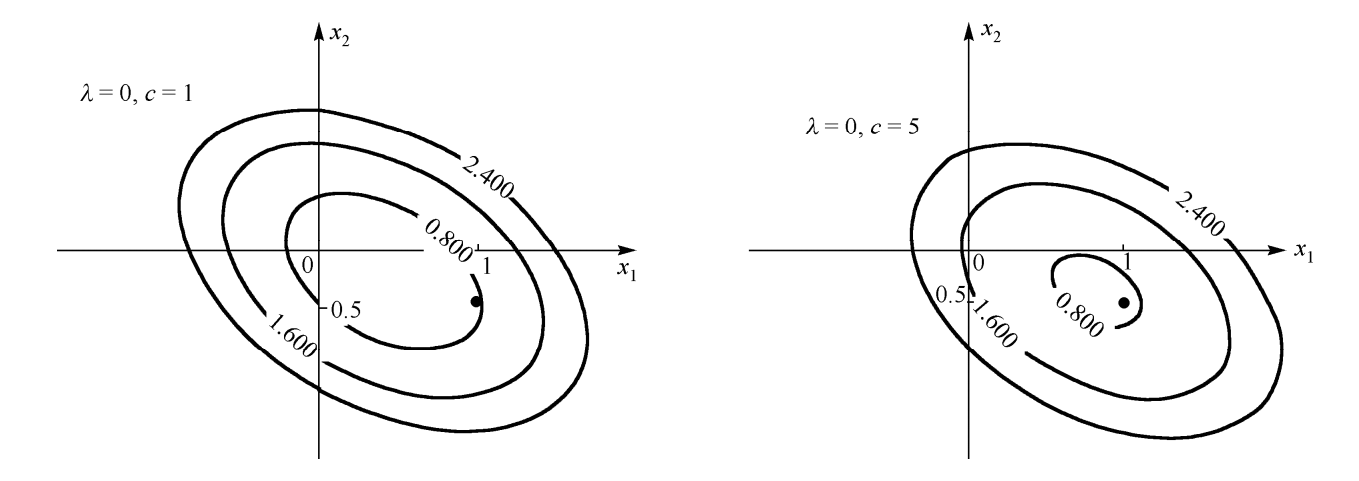
\includegraphics[width=1.0\textwidth]{fig1}
\caption{1 增广拉格朗日函数的等值线}
\end{figure}
\end{frame}


\begin{frame}
%\frametitle{\secname}
$$
L_{c}(x, \lambda)=\frac{1}{2}\left(x_{1}^{2}+x_{2}^{2}\right)+\lambda\left(x_{1}-1\right)+\frac{c}{2}\left(x_{1}-1\right)^{2}
$$
对于 $c=1$和两个不同的 $\lambda$.  $L_{c}(x, \lambda)$的无约束最小值 接近约束最小值$x^{*}=(1,0)$ 当 $\lambda \rightarrow \lambda^{*}=-1$\\
\begin{equation}\tag{2}
	x_{1}(\lambda, c)=\frac{c-\lambda}{c+1}, \quad x_{2}(\lambda, c)=0
\end{equation}
利用 Eq. (2), 我们得到对于所有 $\lambda$,
$$
\lim _{c \rightarrow \infty} x_{1}(\lambda, c)=1=x_{1}^{*}, \quad \lim _{c \rightarrow \infty} x_{2}(\lambda, c)=0=x_{2}^{*}
$$
表明随着 $c$ 的增加, 无约束最小值 $L_{c}(x, \lambda)$ 接近约束最小值。(如图2).
\end{frame}

\begin{frame}
%\frametitle{\secname}
\begin{figure}
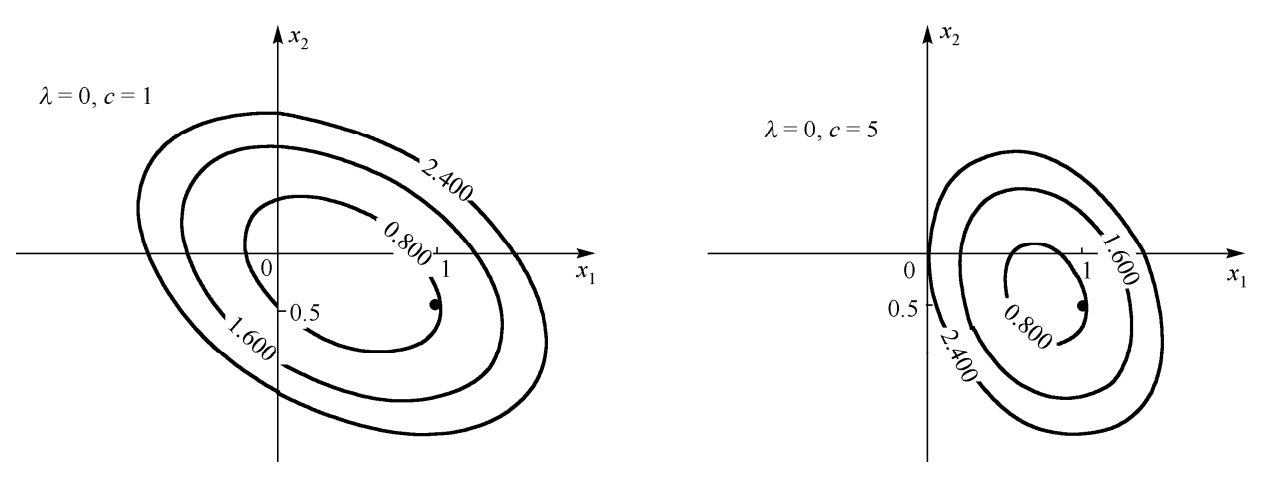
\includegraphics[width=1.0\textwidth]{fig2}
\caption{2 增广拉格朗日函数的等值线}
\end{figure}
\end{frame}

\begin{frame}
%\frametitle{\secname}
$$
L_{c}(x, \lambda)=\frac{1}{2}\left(x_{1}^{2}+x_{2}^{2}\right)+\lambda\left(x_{1}-1\right)+\frac{c}{2}\left(x_{1}-1\right)^{2}
\bigskip
$$
对于示例 , 当$\lambda=0$且两个不同的值$c .$ $L_{c}(x, \lambda)$的无约束最小值 接近约束最小值$x^{*}=(1,0)$当 $c \rightarrow \infty$.
\end{frame}



\subsection{ 二次惩罚函数法 }

\begin{frame}

\frametitle{二次惩罚函数法}
\normaltitle{二次惩罚函数法}
 %is motivated by the preceding considerations. It consists of

它求解一系列如下形式的问题
\begin{center}
$\operatorname{minimize} \quad L_{c^{k}}\left(x, \lambda^{k}\right)$, subject to $x \in X$
\end{center}
 $\left\{\lambda^{k}\right\}$ 是 $\mathbf{R}^{m}$ 中的一个序列, $\left\{c^{k}\right\}$ 是一个正惩罚参数序列, $c^{k}\rightarrow\infty$  
\end{frame}

\begin{frame}
\frametitle{定理}


\textbf{定理2 [收敛]} 假设$f$和$h$是连续函数,$X$是闭集, 约束集 $\{x \in X \mid h(x)=0\}$ 非空. 对于 $k=0,1, \ldots$, 设 $x^{k}$ 为如下问题的全局最优解
\begin{equation}
		\begin{array}{ll}
		\text{ minimize } & L_{c^{k}}\left(x, \lambda^{k}\right) \\
		\text { subject to } &x \in X\\		
		\end{array}
	\end{equation}
其中 $\left\{\lambda^{k}\right\}$ 是有界的, $0<\mathrm{c}^{k}<c^{k+1}$ ,且 $\mathrm{c}^{k} \rightarrow \infty$.

$\Rightarrow$  序列$\left\{x^{k}\right\}$的每个极限点都是原问题的全局最优解。
\end{frame}


\begin{frame}
\frametitle{证明}
\normaltitle			{证明:}\\
令 $\bar{x}$ 是序列 $\left\{x^{k}\right\}$的极限. 根据 $x^{k}$的定义,有
\begin{equation}\label{eq4-23}
L_{c^{k}}\left(x^{k}, \lambda^{k}\right) \leq L_{c^{k}}\left(x, \lambda^{k}\right), \quad \forall x \in X
\end{equation}
记 $f^{*}$ 为原问题 (1)式的最优值,则有
$$
\begin{aligned}
f^{*} &=\inf _{h(x)=0, x \in X} f(x) \\
&=\inf _{h(x)=0, x \in X}\left\{f(x)+\lambda^{k^{\prime}} h(x)+\frac{\mathrm{c}^{k}}{2}\|h(x)\|^{2}\right\} \\
&=\inf _{h(x)=0, x \in X} L_{c^{k}}\left(x, \lambda^{k}\right)
\end{aligned}
$$
\end{frame}

\begin{frame}

%\frametitle{\subsecname}
因此,通过取Eq. (\ref{eq4-23})式右边在条件  $x \in X, h(x)=0$的下界,得:
$$
L_{c^{k}}\left(x^{k}, \lambda^{k}\right)=f\left(x^{k}\right)+\lambda^{k^{\prime}} h\left(x^{k}\right)+\frac{c^{k}}{2}\left\|h\left(x^{k}\right)\right\|^{2} \leq f^{*} .
$$
因为序列 $\left\{\lambda^{k}\right\}$ 是有界的 $\Rightarrow$
  所以该序列有极限 $\bar{\lambda}$.

  不失一般性,假设 $\lambda^{k} \rightarrow \bar{\lambda}$.
\end{frame}


\begin{frame}																				
												
在上述不等式两边取上极限,利用 $f$ 和 $h$ 的连续性:
\begin{equation}\label{eq04}
f(\bar{x})+\bar{\lambda}^{\prime} h(\bar{x})+\limsup _{k \rightarrow \infty} \frac{c^{k}}{2}\left\|h\left(x^{k}\right)\right\|^{2} \leq f^{*}
\end{equation}
因为 $\left\|h\left(x^{k}\right)\right\|^{2} \geq 0$ 且 $c^{k} \rightarrow \infty$, 由此得出 $h\left(x^{k}\right) \rightarrow 0$且
\begin{equation}\label{eq05}
h(\bar{x})=0,
\end{equation}
 Eq.\,(\ref{eq04})式的左边将等于正无穷,而  $f^{*}<\infty$ (因为约束集是非空的),两者相矛盾.

  由于$X$是闭集  $\Rightarrow$ $\bar{x} \in X  $
  $\Rightarrow$故 $\bar{x}$ 是可行的.

  根据Eq  (\ref{eq04}) 和 $(\ref{eq05})$ $\Rightarrow$ $f(\bar{x}) \leq f^{*}$ $\Rightarrow$ $\bar{x}$ 是最优的.   
\end{frame}

\begin{frame}
\frametitle{拉格朗日乘子估计-不精确最小化}
\normaltitle{命题1}\\
假定\hint{增广拉格朗日函数的最小值能被精确地计算出。} 

 %On the other hand, unconstrained minimization methods are usually terminated when the cost gradient is sufficiently small, but not necessarily zero.

 特别地,当$X=\mathbf{R}^{n}$, $f$ 和 $h$ 都可微时,对于如下无约束优化问题

     \begin{equation}
		\begin{array}{ll}
		\text{ minimize } & \quad L_{c^{k}}\left(x, \lambda^{k}\right) \\
		\text { subject to } &x \in \mathbf{R}^{n}\\
		
		\end{array}
	\end{equation}
算法通常会在 $x^{k}$满足
$$
\left\|\nabla_{x} L_{c^{k}}\left(x^{k}, \lambda^{k}\right)\right\| \leq \epsilon^{k}
$$
时终止,其中 $\epsilon^{k}$是一个非常小的量.
\end{frame}

\begin{frame}
\frametitle{定理}
\textbf{定理 3:}
\begin{itemize}
  \item
假定  $X=\Re^{n}$,   $f,h$:都是连续可微的.

\item 令 $k=0,1, \ldots$,  \dred{$x^{k}$ 满足
$
\left\|\nabla_{x} L_{c^{k}}\left(x^{k}, \lambda^{k}\right)\right\| \leq \epsilon^{k}
$}

其中 \hint{$\left\{\lambda^{k}\right\}$ 是有界的;}
\item $\left\{\epsilon^{k}\right\}$ 和 $\left\{c^{k}\right\}$ 满足
$$
\begin{array}{c}
0<c^{k}<c^{k+1}, \quad \forall k, \quad c^{k} \rightarrow \infty \\
0 \leq \epsilon^{k}, \quad \forall k, \quad \epsilon^{k} \rightarrow 0
\end{array}
$$
\item 假设子序列$\left\{x^{k}\right\}_{K}$收敛到向量 $ x^{*}$x* : 且$\nabla h\left(x^{*}\right)$ 的秩为$m$.
   \end{itemize}
    $\Rightarrow$
    \begin{itemize}
      \item
$
 \hspace{7ex}
\hint{\left\{\lambda^{k}+c^{k} h\left(x^{k}\right)\right\}_{K} \rightarrow \lambda^{*}}
$

\item 其中向量$\lambda^{*}$和 $x^{*}$满足一阶必要条件
$$
\dred{\nabla f\left(x^{*}\right)+\nabla h\left(x^{*}\right) \lambda^{*}=0, \quad h\left(x^{*}\right)=0}
$$
    \end{itemize}
\end{frame}

\begin{frame}
\frametitle{证明}
\textbf{证明:}\\
不失一般性,我们假设整个序$\left\{x^{k}\right\}$收敛到$x^{*}$ ,对于所有$k$ ,定义 
$$
\tilde{\lambda}^{k}=\lambda^{k}+c^{k} h\left(x^{k}\right)
$$
那么有
\begin{equation}
\nabla_{x} L_{c^{k}}\left(x^{k}, \lambda^{k}\right)=\nabla f\left(x^{k}\right)+\nabla h\left(x^{k}\right)\left(\lambda^{k}+c^{k} h\left(x^{k}\right)\right)=\nabla f\left(x^{k}\right)+\nabla h\left(x^{k}\right) \tilde{\lambda}^{k}
\end{equation}
因为$\nabla h\left(x^{*}\right)$的秩为 $m$, 所以对充分大的 $k$,$\nabla h\left(x^{k}\right)$的秩也为 $m$. 不失一般性,假设
对于所有$k $,$\nabla h\left(x^{k}\right)$的秩都为 $m$.然后对Eq. $(6)$式两边同时左乘
$$
\left(\nabla h\left(x^{k}\right)^{\prime} \nabla h\left(x^{k}\right)\right)^{-1} \nabla h\left(x^{k}\right)^{\prime}
$$
\end{frame}

\begin{frame}
得到
\begin{equation}
\tilde{\lambda}^{k}=\left(\nabla h\left(x^{k}\right)^{\prime} \nabla h\left(x^{k}\right)\right)^{-1} \nabla h\left(x^{k}\right)^{\prime}\left(\nabla_{x} L_{c^{k}}\left(x^{k}, \lambda^{k}\right)-\nabla f\left(x^{k}\right)\right)
\end{equation}
因为假设 $\nabla_{x} L_{c^{k}}\left(x^{k}, \lambda^{k}\right) \rightarrow 0$, 所以根据Eq. $(7)$式, 有
$$
\tilde{\lambda}^{k} \rightarrow \lambda^{*}
$$
其中
$$
\lambda^{*}=-\left(\nabla h\left(x^{*}\right)^{\prime} \nabla h\left(x^{*}\right)\right)^{-1} \nabla h\left(x^{*}\right)^{\prime} \nabla f\left(x^{*}\right)
$$
再次利用 $\nabla_{x} L_{c^{k}}\left(x^{k}, \lambda^{k}\right) \rightarrow 0$ 和Eq. (6),得到
$$
\nabla f\left(x^{*}\right)+\nabla h\left(x^{*}\right) \lambda^{*}=0
$$
因为序列$\left\{\lambda^{k}\right\}$是有界的,且 $\lambda^{k}+c^{k} h\left(x^{k}\right) \rightarrow \lambda^{*}$,所以 $\left\{c^{k} h\left(x^{k}\right)\right\}$
也是有界的. 因为 $c^{k} \rightarrow \infty$, 所以 $h\left(x^{k}\right) \rightarrow 0$ 故 $h\left(x^{*}\right)=0 .$ 
\end{frame}

\begin{frame}
\frametitle{关于条件数较大的问题}

现在考虑二次惩罚法的实际应用 $\mathrm{p}$ 假设第$k$次迭代中 $L_{c^{k}}($ 对应的无约束最小化问题
在
$$
\left\|\nabla_{x} L_{c^{k}}\left(x^{k}, \lambda^{k}\right)\right\| \leq \epsilon^{k}
$$
时结束
其中 $\epsilon^{k} \rightarrow 0$. 那么有三种可能:\\
\qquad (a) 没有满足$
\left\|\nabla_{x} L_{c^{k}}\left(x^{k}, \lambda^{k}\right)\right\| \leq \epsilon^{k}
$的 $x^{k}$存在,该方法失效.\\
\qquad 情况(a)经常在  $L_{c^{k}}\left(\cdot, \lambda^{k}\right)$ 无界时发生.\\
\end{frame}

\begin{frame}

\qquad (b)满足 $\left\|\nabla_{\mathbf{x}} L_{c_k}\left(\boldsymbol{x}_k, \lambda_k\right)\right\| \leqslant \epsilon_k$ 的序列 $\left\{\boldsymbol{x}_k\right\}$ 存在, 但该序列要么没有极限, 要么它的极限 $\boldsymbol{x}_*$ 使 矩阵 $\nabla h\left(\boldsymbol{x}_*\right)$ 具有线性相关的列 (不满足列满秩条件).\\
\qquad 情况(b)通常在 $L_{c^{k}}\left(\cdot, \lambda^{k}\right)$ 有界时发生, 但原问题没有可行解。
\end{frame}

\begin{frame}

\qquad (c)满足 $\left\|\nabla_{\mathbf{x}} L_{c_k}\left(\boldsymbol{x}_k, \lambda_k\right)\right\| \leqslant \epsilon_k$ 的序列 $\left\{\boldsymbol{x}_k\right\}$ 存在, 且极限 $\boldsymbol{x}_*$ 使矩阵 $\nabla h\left(\boldsymbol{x}_*\right)$ 的秩为 $m$ 。根据命题,$ \boldsymbol{x}_*$ 和 $\lambda_*$ 满足最优化问题的一阶必要条件.\\
\qquad 情况 (c) 是最常见的,无约束最小化算法对于每个$k$都成功找到最优解,通常情况下$\left\{\boldsymbol{x}_k\right\}$收敛到一个可行解;当然, $\left\{\boldsymbol{x}_k\right\}$收敛到局部最优解$x^{*}$是有可能的。那么,如果$x^{*}$不存在对应的拉格朗日乘子向量,则序列$\left\{\lambda^{k}+c^{k} h\left(x^{k}\right)\right\}$发散且没有极限。
\end{frame}

\begin{frame}
\frametitle{实践表明}
惩罚函数法:\\
\qquad (1) 在总体上是相当可靠的\\
\qquad (2) 通常收敛于原问题的局部最优解.\\

\end{frame}

\begin{frame}
当它失效时,通常是由于随着$c^{k} \rightarrow \infty$,最小化如下子问题的难度越来越大
$$
\text { minimize } L_{c^{k}}\left(x, \lambda^{k}\right)
$$
\centerline{subject to $x \in X$}
\\
\qquad  假设 $\boldsymbol{X}=\mathbf{R}^n, f$ 和 $h$ 都是二次可微的, 那么根据梯度方法的收玫速度, 最小化 的难度取决于 Hessian 矩阵  $\nabla_{x x}^{2} L_{c^{k}}\left(x^{k}, \lambda^{k}\right)$ 的最大特征值与最小特征值之比 (条件数), 且该比 值随 $c_k$ 增大而增大。
\end{frame}

\begin{frame}
\frametitle{示例}
考虑二元函数极小化问题

\begin{equation}
		\begin{array}{ll}
		\text{ minimize } &f(x)=\frac{1}{2}\left(x_{1}^{2}+x_{2}^{2}\right) \\
		\text { subject to } &x_{1}=1\\
		
		\end{array}
	\end{equation}

增广拉格朗日函数为
\begin{equation}
		\begin{array}{ll}
		\text L_{\mathrm{c}}(x, \lambda)=\frac{1}{2}\left(x_{1}^{2}+x_{2}^{2}\right)+\lambda\left(x_{1}-1\right)+\frac{c}{2}\left(x_{1}-1\right)^{2} \\
		
		
		\end{array}
	\end{equation}

其 Hessian 矩阵为
$$
\nabla_{x x}^{2} L_{\mathrm{c}}(x, \lambda)=I+c\left(\begin{array}{l}
1 \\
0
\end{array}\right)\left(\begin{array}{ll}
1 & 0
\end{array}\right)=\left(\begin{array}{cc}
1+c & 0 \\
0 & 1
\end{array}\right)
$$
\end{frame}

\begin{frame}
\qquad 该矩阵的特征值分别为$1+c$ 和 1,因此,Hessian 矩阵的最大特征值与最小特征值之比为$1+c$ 。当$c$趋于正无穷时,该比值也趋于正无穷。对于较大的$c$,其增广拉格朗日函数具有较窄水平集,可知函数是病态的。\\
\end{frame}




 \subsection{ 乘子方法的主要思想 }

\begin{frame}
\frametitle{乘子方法的主要思想}
考虑问题
\begin{equation}
		\begin{array}{ll}
		\text{ minimize } &f(x) \\
		\text { subject to } &h(x)=0\\
		
		\end{array}
	\end{equation}

前面提到,在两种情况下可以通过极小化增广拉格朗日函数 $L_{c}(\cdot, \lambda)$,很好地近似这个问题的最优解:\\
\bigskip
\qquad (a) 向量$\lambda$接近于拉格朗日乘子.\\
\qquad (b) 惩罚参数$c$非常大.
\end{frame}

\begin{frame}
\qquad 除了有界性之外,没有对序列$\left\{\lambda^k\right\}$进行任何假设, 在对$f$和 $h$最小化的假设下,即使 $c_k$ 没有趋近无穷, 通过使用更好的方案更新 $\lambda_k$, 从而缓解了增广 Lagrange函数条件过大的困难,也能显著提高收敛速度。\\
\qquad 在一些合理的假设下,即使$c_k$没有趋近无穷,这种方法也是可行的。
\end{frame}

\begin{frame}
\frametitle{乘子法}
\normaltitle{乘子法}\\
\bigskip
在二次惩罚方法中$\lambda^{k}$的更新公式为
\begin{equation}
\lambda^{k+1}=\lambda^{k}+c^{k} h\left(x^{k}\right) .
\end{equation}
\end{frame}

\begin{frame}
\qquad 如果生成的序列$\{x^k\}$ 收敛到局部最小解 $x^*$ ,那么$\{\lambda^k + c^kh(x^k)\}$ 收敛到相应的拉格朗日乘子向量 $\lambda^*$.\\
\qquad 使用上述$\lambda^{k}$更新公式的二次惩罚法称为\hint{乘子法.}
\end{frame}

\begin{frame}
\frametitle{示例}

再次考虑问题
\begin{equation}
		\begin{array}{ll}
		\text{ minimize } &f(x)=\frac{1}{2}\left(x_{1}^{2}+x_{2}^{2}\right) \\
		\text { subject to } &x_{1}=1\\
		
		\end{array}
	\end{equation}
最优解 $x^{*}=(1,0)$ 对应的拉格朗日乘子 $\lambda^{*}=-1 .$ 增广拉格朗日函数为
$$
L_{\mathrm{c}}(x, \lambda)=\frac{1}{2}\left(x_{1}^{2}+x_{2}^{2}\right)+\lambda\left(x_{1}-1\right)+\frac{c}{2}\left(x_{1}-1\right)^{2}
$$
\end{frame}

\begin{frame}
向量$x^{k}$通过乘子法来最小$L_{\mathrm{c}} k\left(\cdot, \lambda^{k}\right)$,并且可以由下式给出
$$
x^{k}=\left(\frac{c^{k}-\lambda^{k}}{c^{k}+1}, 0\right)
$$
使用该表达式,乘子更新公式(8) 可以写成
$$
\lambda^{k+1}=\lambda^{k}+c^{k}\left(\frac{c^{k}-\lambda^{k}}{c^{k}+1}-1\right)=\frac{\lambda^{k}}{c^{k}+1}-\frac{c^{k}}{c^{k}+1}
$$
或者通过引入拉格朗日乘数 $\lambda^{*}=-1$,
$$
\lambda^{k+1}-\lambda^{*}=\frac{\lambda^{k}-\lambda^{*}}{c^{k}+1}
$$
\end{frame}

\begin{frame}
\frametitle{评述}
(1)对于每一个非递减序列$\left\{\mathrm{c}^{k}\right\}$, $\lambda^{k} \rightarrow \lambda^{*}=-1$ 且 $x^{k} \rightarrow x^{*}=(1,0)$  因为 $1 /\left(c^{k}+1\right)$ 乘 $\lambda^{k}-\lambda^{*}$ 总是小于1。\\
(2)$c^{k}$越大,收敛速度越快:事实上,如果$c^{k} \rightarrow \infty$,$\left\{\mid \lambda^{k}-\right.$ $\left.\lambda^{*} \mid\right\}$是超线性收敛的。\\
(3) 当然,我们没有必要让$c^{k}$趋近无穷,尽管这样做能提高收敛速度。
%, although doing so results in a better convergence rate.


\end{frame}




\begin{frame}
\frametitle{作业}

\bigskip
\centering
利用乘子法
$\text { minimize } f(x)=x_{1}^{2}+x_{1}x_{2}+x_{2}^{2}$, subject to $x_{1}=1$\\

\end{frame}



%\end{CJK*}
\end{document}
